%This work is licensed under the Creative Commons
%Attribution-ShareAlike 4.0 International License. To view a copy of
%this license, visit http://creativecommons.org/licenses/by-sa/4.0/ or
%send a letter to Creative Commons, PO Box 1866, Mountain View, CA
%94042, USA.

%This work is licensed under the Creative Commons
%Attribution-ShareAlike 4.0 International License. To view a copy of
%this license, visit http://creativecommons.org/licenses/by-sa/4.0/ or
%send a letter to Creative Commons, PO Box 1866, Mountain View, CA
%94042, USA.

%\documentclass[gray,handout, pdftex, 11pt]{beamer}
%\documentclass[handout, pdftex, 11pt]{beamer}

\documentclass[pdftex, 11pt]{beamer}

\usepackage[utf8]{inputenc}
\usepackage[T1]{fontenc}
\usepackage{lmodern}
%\usepackage[italian]{babel}
\usepackage{acronym}
\usepackage{graphicx}
\usepackage{multirow}
\usepackage{listings}
\usepackage{microtype}
\usepackage{acronym}
\usepackage{array}
\usepackage{tikz}
\usetikzlibrary{shapes, chains, scopes, shadows, positioning, arrows,
  decorations.pathmorphing, calc}

\colorlet{c1}{green!20}
\colorlet{c2}{blue!10}
\colorlet{c3}{yellow!10}
\colorlet{c4}{red!10}
\colorlet{drawColor}{black!50}
\colorlet{commentColor}{green!70!black!90}
\colorlet{codeBgColor}{yellow!50}
\colorlet{bashBgColor}{green!50}

\tikzstyle{oval}=[ellipse, align=center, drop shadow, draw=drawColor, fill=white]
\tikzstyle{rect}=[rectangle, rounded corners=2pt, align=center, drop
shadow, draw=drawColor, fill=white]
\tikzstyle{comment}=[text=commentColor,font=\itshape]
\tikzstyle{textLab}=[]
\tikzstyle{arrow}=[->, very thick, >=stealth', draw=black!80]
\tikzstyle{darrow}=[->, dash pattern=on 3pt off2pt, very thick, >=stealth', draw=black!80]
\tikzstyle{fInt}=[circle, align=center, drop shadow, draw=drawColor, fill=white]
\tikzstyle{fStartEnd}=[ellipse, align=center, drop shadow, draw=drawColor, fill=white]
\tikzstyle{fInput}=[trapezium, trapezium left angle=70, trapezium right angle=110,
align=center, drop shadow, draw=drawColor, fill=white]
\tikzstyle{fProcess}=[rectangle, align=center, drop shadow, draw=drawColor, fill=white]
\tikzstyle{fSelection}=[diamond, shape aspect=3, align=center, drop
shadow, draw=drawColor, fill=white]
\tikzstyle{fOutput}=[tape, tape bend top=none, align=center, drop shadow, draw=drawColor, fill=white]
\tikzstyle{mem}=[rectangle, align=center, draw=drawColor, fill=white]
\tikzstyle{clo}=[cloud, aspect=2, align=center, drop shadow, draw=drawColor, fill=white]
\tikzstyle{file}=[chamfered rectangle, chamfered rectangle corners =
north east, align=center, drop shadow, draw=drawColor, fill=white]
\tikzstyle{files}=[chamfered rectangle, chamfered rectangle corners = north east, align=center, double copy shadow, draw=drawColor, fill=white]

\lstdefinestyle{customJava}{
   language=Java,
   % basicstyle=\small\ttfamily\bfseries,
   basicstyle=\ttfamily,
   keywordstyle=\color{blue}\ttfamily,
   stringstyle=\color{red}\ttfamily,
   commentstyle=\color{green}\ttfamily,
   morecomment=[l][\color{magenta}]{\#},
   % breaklines=false,
   breaklines=true, breakatwhitespace=false,
   postbreak=\raisebox{0ex}[0ex][0ex]{\ensuremath{\color{red}\hookrightarrow\space}},
   frameround=fttt,
   frame=trBL,
   backgroundcolor=\color{yellow!20},
   numbers=left,
   stepnumber=1,    
   firstnumber=1,
   numberfirstline=true,
   numberstyle=\tiny\color{black!50},
   xleftmargin=2em,
   framexleftmargin=1.5em,
   % rulesepcolor=\color{gray},
   rulecolor=\color{black}
   % linewidth=8cm,
}

\lstdefinestyle{customBash}{
   language=bash,
   % basicstyle=\small\ttfamily\bfseries,
   basicstyle=\ttfamily,
   keywordstyle=\color{blue}\ttfamily,
   stringstyle=\color{red}\ttfamily,
   commentstyle=\color{green}\ttfamily,
   morecomment=[l][\color{magenta}]{\#},
   % breaklines=false,
   breaklines=true, breakatwhitespace=false,
   postbreak=\raisebox{0ex}[0ex][0ex]{\ensuremath{\color{red}\hookrightarrow\space}},
   frameround=fttt,
   frame=trBL,
   backgroundcolor=\color{green!20},
   numbers=left,
   stepnumber=1,    
   firstnumber=1,
   numberfirstline=true,
   numberstyle=\tiny\color{black!50},
   xleftmargin=2em,
   framexleftmargin=1.5em,
   % rulesepcolor=\color{gray},
   rulecolor=\color{black}
   % linewidth=8cm,
}

\lstnewenvironment{jblock}[1][]
{
  \lstset{
    style=customJava,
    #1
  }
}{}

\newcommand{\jfile}[2][]{
  \lstinputlisting[style=customJava, title={\texttt{\detokenize{#2}}}, #1]{#2}
}

\newcommand{\jj}[2][]{\lstinline[style=customJava,#1]`#2`}
  %\colorbox{codeBgColor}{
  %  \lstinline[style=customJava,#1]`#2`
  %}
%}

\lstnewenvironment{bblock}[1][]
{
  \lstset{
    style=customBash,
    #1
  }
}{}

\newcommand{\bfile}[2][]{
  \lstinputlisting[style=customBash, title={\texttt{\detokenize{#2}}}, #1]{#2}
}

\newcommand{\bb}[2][]{
  \colorbox{bashBgColor}{
    \lstinline[style=customBash,#1]`#2`
  }
}

\graphicspath{{img/}}
\lstset{inputpath=../cSrc/}

\newcommand{\me}{\mathrm{e}}
\newcommand{\C}{\texttt{C}}
\newcommand{\gcc}{\texttt{gcc}}
\newcommand{\bash}{\texttt{Bash}}

\definecolor{links}{HTML}{2A1B81}
\hypersetup{colorlinks,linkcolor=links,urlcolor=links}

\definecolor{links}{HTML}{2A1B81}
\hypersetup{colorlinks,linkcolor=,urlcolor=links}


\mode<presentation>{
  %-------------------------1
  \usetheme{Boadilla}
  \usecolortheme{beaver}
  %-------------------------1
  %-------------------------2
  %\usetheme{Goettingen}
  %\usecolortheme{sidebartab}
  %-------------------------2
  %\useoutertheme[right]{sidebar}
  %\usefonttheme{default}
  \setbeamercovered{transparent}
  %\setbeameroption{show notes on second screen=right}
  \setbeamertemplate{navigation symbols}{}
  \setbeamertemplate{footline}{}

  \bibliographystyle{abbrv}  
  %\renewcommand\bibfont{\scriptsize}
  \setbeamertemplate{bibliography item}{\textbullet}
  \setbeamertemplate{itemize item}{\checkmark}
  \setbeamertemplate{itemize subitem}{-}
  \setbeamertemplate{enumerate items}[default]
  \setbeamertemplate{sections/subsections in toc}[square]
}



\begin{document}

\title[\acs{MRP} steady-state]{\textbf{\acl{MRP} -
    steady-state analysis}}
\date[\today]{\flushright \today}
\subtitle{MVT exam}
\institute[Uni. Firenze]{
%  
\includegraphics[width=2cm]{img/logoUnifi.eps}\\
  
\includegraphics[width=2cm]{img/logoUnifi.png}\\
  Universit\`a degli Studi di Firenze
}

\author[Martina - Papini]{
  \begin{center}
    \begin{tabular}{lr}
      Stefano \textsc{Martina}&Tommaso \textsc{Papini}\\
      \href{mailto:stefano.martina@stud.unifi.it}{stefano.martina@stud.unifi.it}&
      \href{mailto:tommaso.papini1@stud.unifi.it}{tommaso.papini1@stud.unifi.it}
    \end{tabular}
  \end{center}
}

\titlegraphic{
  \vspace{-0.5cm}
  \tiny
  \href{http://creativecommons.org/licenses/by-sa/4.0/}{
\includegraphics[width=1cm]{img/logoCC.png}}
  This work is licensed under a
  \href{http://creativecommons.org/licenses/by-sa/4.0/}{Creative
    Commons Attribution-ShareAlike 4.0 International License}.
}

\newacro{MRP}{Markov Regenerative Process}
\newacro{SMP}{Semi-Markov Process}
\newacro{CTMC}{Continuous Time Markov Process}
\newacro{DTMC}{Discrete Time Markov Process}
\newacro{PN}{Petri Net}

\acrodefplural{MRP}[MRPs]{Markov Regenerative Processes}
\acrodefplural{SMP}[SMPs]{Semi-Markov Processes}
\acrodefplural{CTMC}[CTMCs]{Continuous Time Markov Processes}
\acrodefplural{DTMC}[DTMCs]{Discrete Time Markov Processes}
\acrodefplural{PN}[PNs]{Petri Nets}

\begin{frame}[plain]
  \titlepage
\end{frame}

\section{Intro \acfp{MRP}}
\begin{frame}
  \frametitle{\acfp{MRP}}
  \begin{block}{Definition}
    A \acf{MRP} is a stochastic process that sooner or later, with
    probability one, will
    reach a \alert{regenerative} state (will be regenerated).
  \end{block}
  \pause
  \begin{block}{Regenerative state}
    A state where the process loses its memory. 
  \end{block}
  \pause
  \begin{center}    
    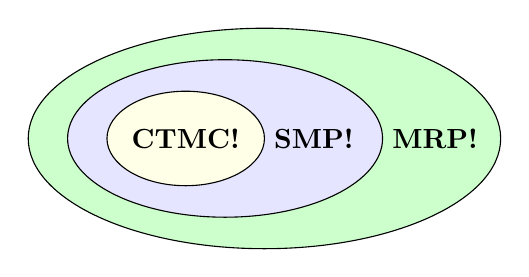
\begin{tikzpicture}[node distance=5mm]
      \visible<5->{\draw[fill=c1] (1,0) ellipse (3cm and 1.4cm)  node[right=1.5cm] {\acs{MRP}};}
      \visible<4->{\draw[fill=c2] (0.5,0) ellipse (2cm and 1cm) node[right=.5cm] {\acs{SMP}};}
      \visible<3->{\draw[fill=c3] (0,0) ellipse (1cm and 0.6cm) node {\acs{CTMC}};}
    \end{tikzpicture}
  \end{center}
\end{frame}

\begin{frame}
  \frametitle{The steady-state problem}
  \pause
  \begin{block}{Transient probabilities}
    The probability distribution that the process will be in a certain
    state, after given $t$ time.
  \end{block}
  \pause
  \begin{block}{Steady-state}
    For ergodic systems, it represents the probability distribution
    that the
    process will be in a certain state, as time goes to infinity.
  \end{block}
  \pause
  \begin{itemize}
  \item ORIS current state:
    \begin{itemize}
    \item Transient analysis for \acfp{MRP}
    \item Steady-state analysis for \acfp{CTMC}
    \end{itemize}
    \pause
  \item Until now! \rotatebox[origin=c]{270}{:D}
    \pause
  \item \alert{Warning:} we assume that the \acs{MRP} is ergodic!
  \end{itemize}
\end{frame}

\section{General algorithm}
\begin{frame}
  \frametitle{\acs{MRP} steady-state analysis - The theory}
  General idea:
  \begin{enumerate}
  \item<2-> Calculate the embedded \acs{DTMC} steady-state on the
    regenerative states
  \item<3-> Calculate the expected sojourn time in each marking, after
    reaching a regenerative state
  \item<4-> Combine the two above in order to calculate the \acs{MRP} steady-state
  \end{enumerate}
  \begin{center}
    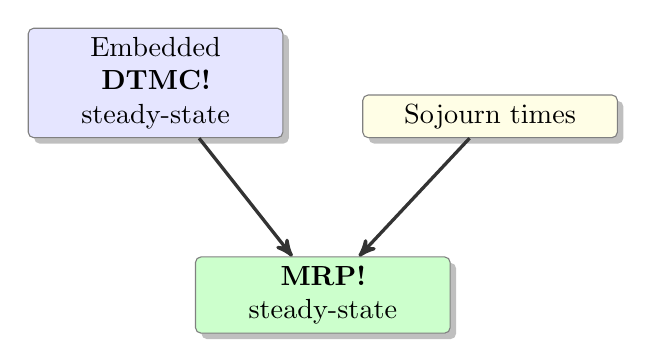
\begin{tikzpicture}[node distance=1.5cm and 5mm, text width=3cm, align=center]
      \uncover<4->{\node (combine) [rect, fill=c1] {\acs{MRP} steady-state};}
      \uncover<2->{\node (embedded) [rect, fill=c2, above left=of combine.north] {Embedded \acs{DTMC} steady-state};}
      \uncover<3->{\node (sojourn) [rect, fill=c3, above right=of combine.north] {Sojourn times};}
      \uncover<4->{\draw[arrow] (embedded) -- (combine);}
      \uncover<4->{\draw[arrow] (sojourn) -- (combine);}
    \end{tikzpicture}
  \end{center}
\end{frame}

\subsection{Main classes implemented}
\begin{frame}
  \frametitle{\insertsubsection}
  \begin{itemize}
	  \item \jj{class EmbeddedDTMC}
	  %\pause
	  \begin{itemize}
	  	\item written from scratch
	  	\item calculate embedded \acs{DTMC} steady-state
	  \end{itemize}
	  %\pause
	  \item \jj{class RegenerativeSteadyStateAnalysis}
	  %\pause
	  \begin{itemize}
	  	\item based on \jj{class RegenerativeTransientAnalysis}
	  	\item calculate \acs{MRP} steady-state
	  \end{itemize}
  \end{itemize}
\end{frame}

\subsection{Steady-state of the embedded \acs{DTMC} on regenerative
  states}
\begin{frame}
  \frametitle{\insertsubsection}
  \begin{block}{Steady-state in \acf{DTMC}}
    If the steady-state of a \acf{DTMC} exists and is unique (if is
    ergodic), then it's calculated by solving for $v$ the linear
    system:
    \begin{equation*}
      \begin{cases}
        v=vP\\
        |v| = 1
      \end{cases}
    \end{equation*}
  \end{block}
  \pause
  \begin{itemize}
  \item We want to calculate the steady-state of the embedded \acs{DTMC} of the \acs{MRP} in
    the regenerative states
    \pause
  \item But we don't have $P$! \rotatebox[origin=c]{270}{:(}
  \end{itemize}
\end{frame}

\begin{frame}
  \begin{block}{Reaching probability feature}
    \begin{itemize}
    \item We add a new \alert{reaching probability feature} to each
      state: \jj{class ReachingProbabilityFeature}
      % \pause
    \item Inside \jj{SteadyStateInitialStateBuilder}: set it to
      1
      %\pause
    \item Inside \jj{SteadyStatePostProcessor}: multiply the
      parent's reaching probability by the probability to chose a
      certain child
    \end{itemize}
  \end{block}
  %\pause
  If we run a transient analysis on the \acf{PN} we get:
  \begin{itemize}
  \item \jj{regenerationClasses}
  \item {\scriptsize\jj{Map<DeterministicEnablingState,Map<DeterministicEnablingState,Set<State>>>}}
  \item sum reaching probability feature of each \jj{State} to compute
    elements of \alert{$P$}
  \end{itemize}
\end{frame}

\begin{frame}
  Now we can solve the linear system:
  \begin{equation*}
    \begin{cases}
      v=vP\\
      |v| = 1
    \end{cases}
    =
    \begin{cases}
      (P'-I)v'=0\\
      \sum_i v_i = 1
    \end{cases}
  \end{equation*}
  \begin{itemize}
  \item \jj{RealMatrix} \& \jj{RealVector}
  \item QR decomposition solver
    \begin{itemize}\tiny
    \item \jj{DecompositionSolver solver = new QRDecomposition(coefficients).getSolver();}
    \item \jj{RealVector steadyState = solver.solve(constants);}
    \end{itemize}
  \item Convert \jj{steadyState} into a \jj{Map<DeterministicEnablingState,BigDecimal>}
  \end{itemize}
\end{frame}

\subsection{Sojourn time $a_{ij}$}
\begin{frame}
  \frametitle{\insertsubsection}
  \begin{block}{Definition}
    The sojourn time \alert{$a_{ij}$} represents the average time spent in the
    \alert{$j$-th marking} after the (last) \alert{$i$-th regeneration}.
  \end{block}
\end{frame}

\begin{frame}
  \frametitle{How to compute $a_{ij}$?}
  $a_{ij}$ is:
  \begin{itemize}
  \item sum of avg time spent in marking $j$ occurrences
    \begin{itemize}
    \item sum of avg time before each variable fires
      \begin{itemize}
      \item condition each variable to be the minimum (i.e. the one
        that fires)
      \item compute avg time before that variable fires (thanks Marco!)
      \end{itemize}
    \end{itemize}
  \end{itemize}
  \begin{center}
    \begin{tikzpicture}[myMindmap]
      \begin{scope}[concept color=mmc2]
        \node(l) {i}
        child[concept color=mmcb] { node {}
          child { node{} }
          child[concept color=mmc1] { node{j}
            child[concept color=mmcb] { node{} }
            child[concept color=mmcb] { node{} }
          }
        }
        child[concept color=mmcb] { node{} }
        child[concept color=mmcb] { node{} 
          child[concept color=mmc1] { node{j}
            child[concept color=mmcb] { node {} }
          }
        };        
      \end{scope}
      \begin{scope}[concept color=mmc1]
        \node[right=5cm of l] {j}
        child[concept color=mmcb] { node[label={[label distance=2.5mm]50:$v_1$}] {} }
        child[concept color=mmcb] { node[label={[label distance=0.1mm]93:$v_2$}] {} }
        child[concept color=mmcb] { node[label={[label distance=2.5mm]135:$v_3$}] {} };
      \end{scope}
    \end{tikzpicture}
  \end{center}
\end{frame}

\begin{frame}
  \frametitle{When to compute $a_{ij}$?}
  During the transient analysis!
  \begin{itemize}
  \item transient analysis generates succession trees for each
    regenerative state
    \begin{itemize}
    \item regenerative state as root
    \item following regenerative states as leaves
    \item reachable markings as inner nodes
    \end{itemize}
  \item during the tree generation compute and accumulate $a_{ij}$ for
    each marking occurrence found
  \end{itemize}
\end{frame}
\subsection{\acf{MRP} steady-state}
\begin{frame}
  \frametitle{\insertsubsection}
  Let's combine the embedded \acs{DTMC} steady-state and the sojourn
  times!
  \pause
  \begin{equation*}
    \pi_j = \frac{\sum_i v_i a_{ij}}{K}
  \end{equation*}
  \pause
  \begin{itemize}
  \item We multiply the sojourn time in the marking $j$ after the
    regeneration $i$ by the probability of reaching the $i$-th regeneration
    \pause
  \item We do this for each regeneration that leads to the marking $j$
    before another regeneration
    \pause
  \item $K$ is a normalization factor calculated as the sum of $\pi_j$
  \end{itemize}
\end{frame}
\section{Test}
\begin{frame}
  \frametitle{\insertsection}
  \begin{block}{Unit test}
    \begin{itemize}
    \item Class \jj{SteadyStateTest} with \alert{JUnit} tests
      \pause
    \item Three different models:
      \pause
      \begin{itemize}
      \item TestCaseSMP
        \pause
      \item TestCase2ParallelTasks
        \pause
      \item TestCaseRejuvenation
        \pause
      \end{itemize}
    \item For each test:
      \pause
      \begin{enumerate}
      \item launch \acs{MRP} steady state \alert{analysis}
        \pause
      \item check if the result is comparable to the \alert{expected}
        value \pause (with a tolerance)
      \end{enumerate}
    \end{itemize}
  \end{block}
\end{frame}

\begin{frame}
  \frametitle{Rejuvenation}
  \begin{center}
    \begin{tikzpicture}[scale=1.5]
      \clip (-1,-1) rectangle (7,3.5);

      % \draw [help lines] (0,0) grid (6,2);
      \node (pDown) at (0,1) [myPlace, onslide=<15>{tokens=1}, onslide=<15-16>{highlight}, label=225:$P_{down}$] {};
      \node (pUp) at (2,2) [myPlace, onslide=<{1-3,5,11,17}>{tokens=1}, onslide=<{4,5-6,11-12,17}>{highlight}, label=0:$P_{up}$] {};
      \node (pFprob) at (2,0) [myPlace, onslide=<{7-9,13}>{tokens=1}, onslide=<{7,10,13-14}>{highlight}, label=0:$P_{fprob}$] {};
      \node (pClock) at (4,2) [myPlace, onslide=<{1,5-7,11-}>{tokens=1}, onslide=<{2,5,8,11}>{highlight}, label=135:$P_{clock}$] {};
      \node (pRej) at (4,0) [myPlace, onslide=<{3,9}>{tokens=1}, onslide=<{3-4,9-10}>{highlight}, label=225:$P_{rej}$] {};

      \node (tUp) at (1,2) [transExpV, onslide=<16-17>{highlight}, label=45:$T_{up}$] {}
      edge[pre, bend right=45] (pDown)
      edge[post] (pUp);
      \node (tDown) at (1,0) [transExpV, onslide=<14-15>{highlight}, label=225:$T_{down}$] {}
      edge[pre] (pFprob)
      edge[preN, bend left=35] (pRej)
      edge[post, bend left=45] (pDown);
      \node (tFprob) at (2,1) [transExpH, onslide=<{6-7,12-13}>{highlight}, label=0:$T_{fprob}$] {}
      edge[pre] (pUp)
      edge[preN, bend left=10] (pRej)
      edge[post] (pFprob);
      \node (tClock) at (4,1) [transDetH, onslide=<{2-3,8-9}>{highlight}, label=225:$T_{clock}$] {}
      edge[pre] (pClock)
      edge[preN, bend right=25] (pDown)
      edge[post] (pRej);
      \node (tRej1) at (5,1) [transExpH, onslide=<10-11>{highlight}, label=315:$T_{rej1}$] {}
      edge[pre, bend left=20] (pRej)
      edge[post, bend right=20] (pClock)
      edge[pre, bend left=90] (pFprob)
      edge[post, bend right=90] (pUp);
      \node (tRej2) at (6,1) [transExpH, onslide=<4-5>{highlight}, label={[label distance=2mm]280:$T_{rej2}$}] {}
      edge[pre, bend left=30] (pRej)
      edge[post, bend right=20] (pClock)
      edge[post, bend right=90] (pUp.north);
      \draw[pre] (tRej2) .. controls (7,0) and (6,5) .. (pUp);
    \end{tikzpicture}
  \end{center}
\end{frame}

\begin{frame}
  \frametitle{Transient analysis}
  \begin{center}
    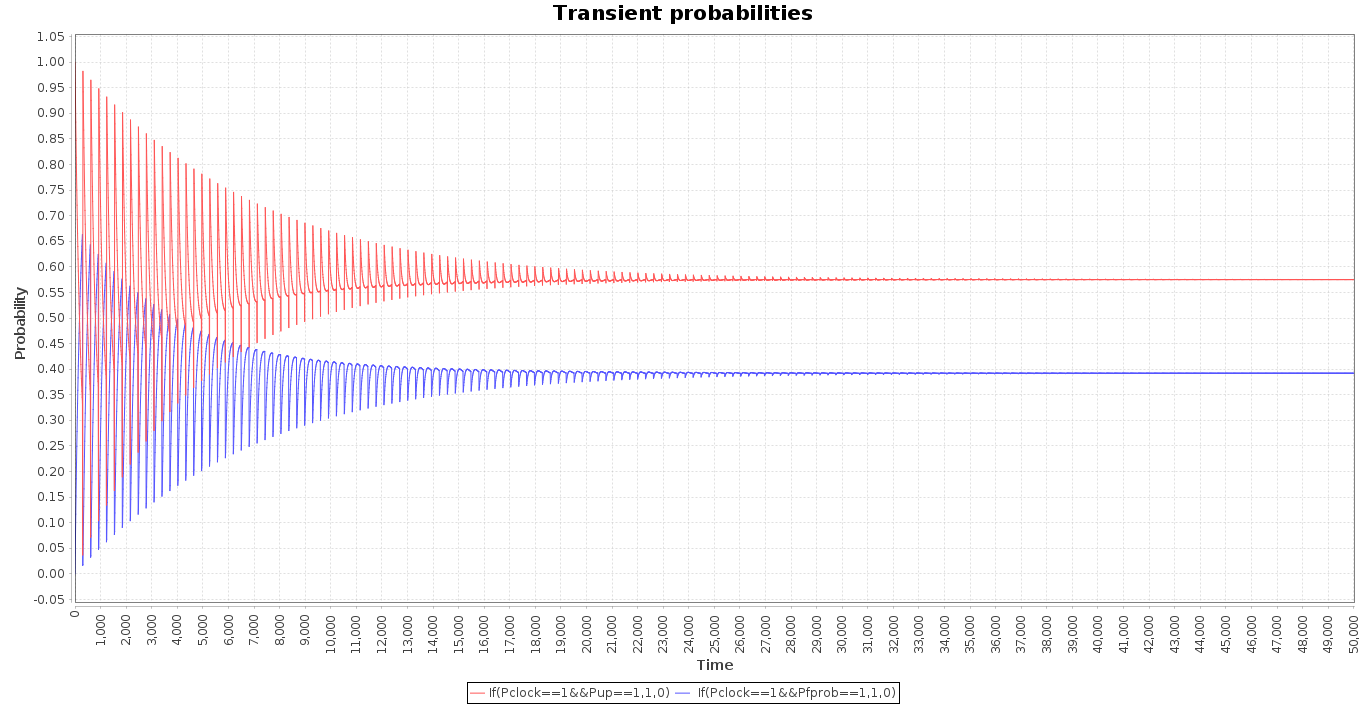
\includegraphics[width=\textwidth]{img/rejuvenationTrans.png}    
  \end{center}
  \pause
  \begin{itemize}
  	\item Steady-state analysis results:
  	\pause
  	\begin{itemize}
  		\item Prob({\color{red} Pclock Pup}) $\approx 0.58$
  		\item Prob({\color{blue} Pclock Pfprob}) $\approx 0.40$
  	\end{itemize}
  \end{itemize}
\end{frame}

\begin{frame}[fragile]
  \frametitle{Steady state analysis}
  \footnotesize
  \begin{jblock}
Map<String, Integer> tmpPlacesMarking = new HashMap<String, Integer>();
tmpPlacesMarking.put("Pup", Integer.parseInt("1"));
tmpPlacesMarking.put("Pclock", Integer.parseInt("1"));
getTestPlacesMarkings().put(tmpPlacesMarking, new BigDecimal("0.58"));

tmpPlacesMarking = new HashMap<String, Integer>();
tmpPlacesMarking.put("Pfprob", Integer.parseInt("1"));
tmpPlacesMarking.put("Pclock", Integer.parseInt("1"));
getTestPlacesMarkings().put(tmpPlacesMarking, new BigDecimal("0.40"));
  \end{jblock}
\end{frame}

\begin{frame}
  \begin{center}
	\textbf{\Huge The End.}\\[3cm]
	\pause
	{\huge questions...?}
  \end{center}
\end{frame}
\end{document}